%%%%%%%%%%%%%%%%%%%%%%%%%%%%%%%%%%%%%%
%%%%%%%%%%%%%%%%%%%%%%%%%%%%%%%%%%%%%%
% Do not edit the TeX file your work
% will be overwritten.  Edit the RnW
% file instead.
%%%%%%%%%%%%%%%%%%%%%%%%%%%%%%%%%%%%%%
%%%%%%%%%%%%%%%%%%%%%%%%%%%%%%%%%%%%%%



On the Iris data, we chose two different functional perturbations: for the first
we let $p_1(\nu_k)$ be a logit normal with parameters $\mu = -2, \sigma = 1$;
for the second, we let $p_1(\nu_k)$ be a logit normal with parameters $\mu = 2,
\sigma = 1$. In both cases, we then chose $\phi(\nu_k) = p_1(\nu_k) /
p_{0k}(\nu_k)$.



\begin{knitrout}
\definecolor{shadecolor}{rgb}{0.969, 0.969, 0.969}\color{fgcolor}\begin{figure}[!h]

{\centering 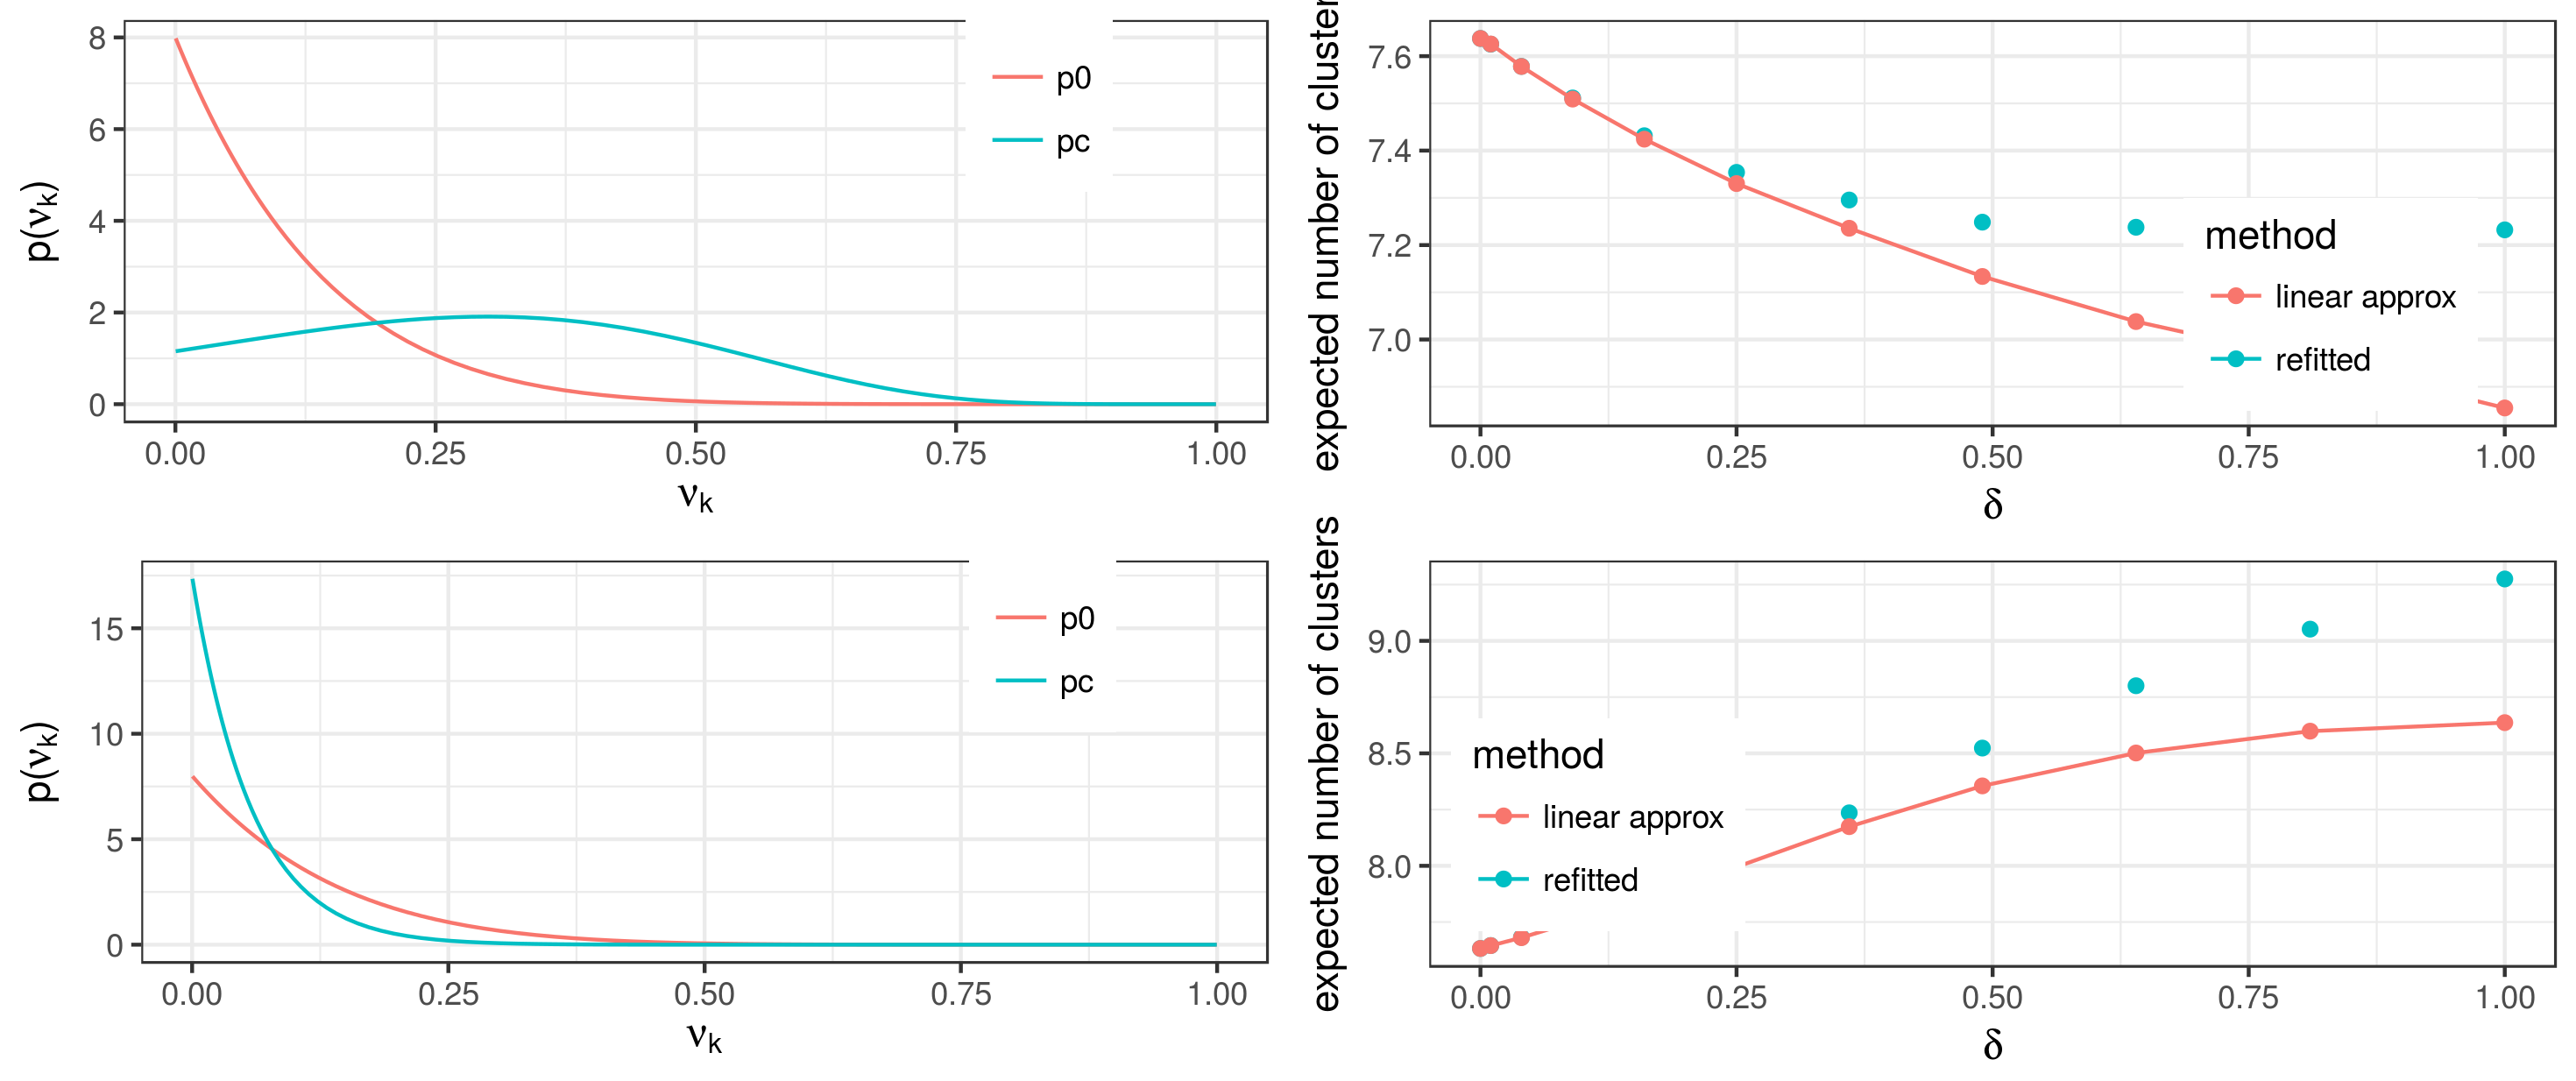
\includegraphics[width=0.98\linewidth,height=0.480\linewidth]{figure/functional_sens_plot-1} 

}

\caption{\label{fig:func_sens_e_num_clusters}
Left column: the original prior $p_{0k}$ in purple,
the perturbed prior $p^c_k$ in red. Right: linearly approximated vs.
re-fitted expected number of clusters after the pertubation.  }\label{fig:functional_sens_plot}
\end{figure}


\end{knitrout}
%
We find that the linear approximation in this case was able to capture the
direction of the perturbation, (expected number of clusters increased under the
first pertubation, decreased under the second), although as
$\delta \rightarrow 1$ the quality of the approximation degraded.
